\documentclass[a4paper, 14pt]{article}
\usepackage{graphicx} % Required for inserting images
\usepackage[margin=1in]{geometry}
\usepackage{parskip}
\usepackage{amsmath,amssymb}
\usepackage{pxfonts}

\newtheorem{prop}{Proposition}
\newtheorem{remark}{Remark}

\title{Adoption of Hydrogen Infrastructure at Airports}
\author{Brett Devine}
\date{August 2024}

\linespread{1.6}

\begin{document}

\maketitle
\thispagestyle{empty}
\begin{abstract}
    I explore the strategic dynamics and network effects involved in aviation's adoption of the technology for sustainable hydrogen-based flight.
    Both the value of hydrogen-based aircraft to airlines and the value of hydrogen infrastructure to airports increase in the mutual adoption of hydrogen.
    I develop best responses for airports and the airline industry in this setting, identify conditions for subgame perfect Nash equilibrium and analyze the results with numerical methods.
    I find that ...
\end{abstract}


% ----------------------------------------------------------
%   BEGIN Airline Demand Model
% ----------------------------------------------------------
\newpage
\section{Introduction}

\section{Airline Demand for Hydrogen}
\label{sec:airline_demand}

The airline industry may wish to adopt hydrogen-fueled aircraft, but will only acquire and use the aircraft if it makes economic sense for them to do so.
Airline demand for hydrogen flight will largely depend upon the costs of hydrogen-fueled passenger miles as well as the amount of passenger miles possible with hydrogen aircraft.
The latter factor is determined by the adoption of hydrogen infrastructure across the airport network to service such aircraft.

Profit maximization for the airline industry requires the efficiency of minimizing the total cost of meeting passenger demand.\footnote{Passenger demand for flight is not explicitly modeled in this paper. This assumes that passengers are indifferent to the fuel or technology used to fly them to their destination as long as the overall experience is equivalent. It also assumes that hydrogen flights will not be priced differently than any other flight, an assumption that would likely hold if consumers are indifferent.}
I model airlines as choosing flight energy inputs to minimize cost subject to meeting passenger flight demand.

Airlines observe the current passenger demand, $Y$, as the passenger miles demanded at current market conditions.
They seek to provide the passenger miles necessary to meet that demand but at the minimum possible cost.
For tractability, I model airports as choosing two input factors to produce passenger miles.
The inputs could be viewed as aircraft, passenger miles capacity, or energy usage.
Airlines choose $K$ as the quantity of JetA or kerosene-based flight (incumbent energy/technology) and $H$ the quantity of hydrogen-based flight to acquire.
Airline input choices of $K$ and $H$ are combined in a CES\footnote{CES stands for constant elasticity of substitution and is very flexible form production function used regularly in economics. Its main feature is that the elasticity of substitution between inputs is held constant across scale of production.} production technology
\begin{align}
    Y(K,H) &= \left( K^{\rho} + SH^{\rho} \right)^{1/\rho} \label{eq:production}
\end{align}
where $S$ is the proportion of airports adopting hydrogen technology and therefore facilitate hydrogen-based passenger miles \footnote{$S$ is the proportion of airports in the network which can service hydrogen aircraft. The potential hydrogen passenger miles are proportional to this number, as the number of connecting flights for a number of airports $S$ is $S(S-1)/2$.} and $\rho \in (0,1)$ is a substitution parameter affecting the elasticity of substitution within the production technology.\footnote{In this case, the elasticity of substitution is viewed as the ability to substitute hydrogen and JetA/Kerosene passenger miles for one another within the production technology.}

Airlines face respective unit prices or costs of $p_K$ and $p_H$ which encapsulate both acquisition cost, service cost, fuel cost, etc for JetA/Kerosene and hydrogen respectively.

After observing market demand $Y$, the airline seeks to solve the problem of choosing $K$ and $H$ to minimize total costs subject to the constraint of meeting demand.
\begin{align}
    \min_{K,H} &\; p_K K + p_H H \nonumber \\
    s.t. &\quad F(K,H) = \left( K^{\rho} + \tilde{S}H^{\rho} \right)^{1/\rho} \geq Y \nonumber \\
    &\quad K\geq 0,\; H\geq 0 \nonumber
\end{align}

To solve the above constrained optimization problem we can view it as an unconstrained problem using Lagrange's technique.
\begin{align}
    \mathcal{L}(K,H,\lambda) = p_k K + p_H H - \lambda(K^{\rho} + \tilde{S} H^{\rho} - Y^{\rho}) \nonumber
\end{align}
The first order conditions for a minimum involve the airline choosing $K$ and $H$ so that their marginal products are equal to their respective marginal costs (price), while simultaneously ensuring demand $Y$ is met exactly.
\begin{align}
    \frac{\partial \mathcal{L}}{\partial K} &= p_K - \lambda \rho K^{\rho-1} = 0 \nonumber \\
    \frac{\partial \mathcal{L}}{\partial H} &= p_H - \lambda \tilde{S}\rho H^{\rho-1} = 0 \nonumber \\
    \frac{\partial \mathcal{L}}{\partial \lambda} &= K^{\rho} + \tilde{S}H^{\rho} - Y = 0 \nonumber
\end{align}
From the above conditions, we can derive the airline's conditional input demand functions which describe for any output level $Y$ and adoption level $S$, the cost minimizing (efficient) choice of $K$ and $H$.
These functions will represent the airline industry's best response to the hydrogen adoption strategies of airports.
\begin{prop}
    The airline industry's input demand functions are
    \begin{align}
        K(p_K,p_H,Y,\tilde{S};\rho) &= Y \left[ \left(\frac{p_H}{p_K}\right)^{\rho/(\rho-1)}\tilde{S}^{-1/(\rho-1)} + 1 \right]^{-1/\rho} \label{eq:K_demand} \\
        H(p_K,p_H,Y,\tilde{S};\rho) &= Y \left[ \left(\frac{p_K}{p_H}\right)^{\rho/(\rho-1)}\tilde{S}^{\rho/(\rho-1)} + \tilde{S} \right]^{-1/\rho} \label{eq:H_demand}
    \end{align}
\end{prop}

Applied use of the airline's demand functions will often require selection of parameter choices.
One such choice, which will be used in equilibrium analysis later, is detailed in the remark below.
\begin{remark}
    Suppose that $\rho = 1/2$.
    Then the airline industry demand function for hydrogen simplifies to
    \begin{align}
        H(p_K,p_H,Y,\tilde{S};1/2) &= Y \left[ \frac{p_K \tilde{S}}{p_H + p_K\tilde{S}^2}. \right]^2 \nonumber
    \end{align}
    By further normalizing the incumbent energy price, $p_K = 1$ we define the price of hydrogen $p_H$ relative to it resulting in demand functions
    \begin{align}
        H(1,p_H,Y,\tilde{S};1/2) &= Y \left[ \frac{\tilde{S}}{p_H + \tilde{S}^2} \right]^2 \nonumber \\
        K(1,p_H,Y,\tilde{S};1/2) &= Y \left[ \frac{p_H}{p_H + \tilde{S}^2} \right]^2 \nonumber
    \end{align}
\end{remark}
The demand functions derived in (\ref{eq:H_demand}) and (\ref{eq:K_demand}) satisfy the typical laws of demand, i.e., that an increase in the own-input price results in a decrease in quantity demanded. Furthermore, demand is observed to increase as $Y$ increases.

% ----------------------------------------------------------
%   BEGIN Airport Model
% ----------------------------------------------------------
\section{Airport Demand for Hydrogen Infrastructure}
\label{sec:airport_demand}
Airports choose infrastructure investments to maximize net present value.
The upfront investment costs of installing the necessary infrastructure to service hydrogen-fueled aircraft must be balanced against the present value of future service revenues.

The primary source of benefits to airports are fees charged to airlines, both terminal fees and aeronautical service fees.
The scale of these fees and their future collectability are proportional to the airport's capacity and the proportion of aircraft or passenger miles fueled by each particular energy source.
Additionally, both the ability to realize airport capacity as well as the ability to command service and terminal fees depends on the airport's connectivity to other airports with matching infrastructure (i.e., conventional or hydrogen).

For a set of $N>1$ airports, the present value of future stream of airport revenues for airport $i=1,\dots, N$ are modeled in perpetuity as shown below.
\begin{align}
    PV_{i} &= \frac{F_K Q_i (1-\alpha)}{\delta - \gamma} + \frac{(F_H S \alpha Q_i}{\delta - \gamma} \cdot A_i \label{eq:gross_PV}
\end{align}
where $F_K$ and $F_H$ are the Kerosene/JetA fees and hydrogen airport fees respectively, each growing at rate $\gamma \geq 0$.
$Q_i$ is the measure of a flight's maximum capacity for flights and $\alpha \in [0,1]$ is the airline industry's proportion of either aircraft or passenger miles demanding hydrogen-based services.
The first term in (\ref{eq:gross_PV}) is the NPV from Kerosene/JetA while the second term represents the NPV from hydrogen services.
The benefits of hydrogen for each airport are affected by $\alpha$ representing the airline industry's demand for hydrogen flight services, as well as by $S$ the number or proportion of airports with hydrogen infrastructure installed.
Finally, $A_i \in \{0,1\}$ is 1 if airport $i$ installs hydrogen infrastructure and is zero otherwise.

Any airport installing hydrogen infrastructure can only benefit if other airports with hydrogen infrastructure exist to provide connecting flights which generate fee revenue.
The more connecting hydrogen flights possible from a given airport, the more valuable an airport's hydrogen services become to airlines and passengers.
For $S < N$ airports with hydrogen infrastructure, the number of connecting hydrogen flights possible are $S(S-1)/2$.
While conventional aircraft are serviceable at every airport and hence can realize $N(N-1)/2$ possible connecting flights.
Hence, the value of hydrogen infrastructure installation for airport $i$ increases as the number of other airports adopting hydrogen increases.

Airport $i$ faces an upfront installation cost of $X_i$, which may be either equal across airports, or scale in proportion to an airport's capacity $Q_i$.
The decision to adopt hydrogen infrastructure will depend on the present value of future benefits exceeding installation costs, or the \textit{net present value}.
Because the benefits from conventional aircraft fees are realized with or without hydrogen infrastructure, they can be removed from the airport's payoff function for strategy selection.
The net payoff for airport $i$'s adoption decision $A_i \in \{0,1\}$ is displayed below.
\begin{align}
    \pi_i(Q_i, X_i, S, A_i) &= \left[ \frac{F_H Q_i}{\delta - \gamma} \cdot \alpha S - X_i \right]A_i, \quad A_i \in \{0,1\} \label{eq:net_PV}
\end{align}
Note that when an airport doesn't adopt ($A_i=0$) the additional net benefits of adoption are zero.
The net present value in (\ref{eq:net_PV}) is the airport's payoff from choosing their strategy $A_i \in \{0,1\}$.
We will see later, that $\alpha$ is a function of $S$ and that since $h(S) = \alpha(S)S$ satisfies the partial derivative condition below, airports will experience network effects when choosing their strategy.
\begin{align}
    \frac{\partial \pi_i(Q_i, X_i, S, A_i)}{\partial h(S)} > 0 \quad&\text{ and }\quad \frac{\partial h(S)}{\partial S} = \alpha'(S)S + \alpha(S) \geq 0 \nonumber
\end{align}

\section{Equilibrium}
\label{sec:equilibrium}
Airports and airlines engage in a two-stage game.
In the first stage, a nonempty set of airports choose simultaneously whether to adopt hydrogen technology or not.
In the second stage, airlines choose the mix of conventional and hydrogen-fueled flights in best response (i.e., minimize costs) to the adoption or non-adoption strategy of airports.
With common knowledge, each player is aware of the distribution of airport sizes, the aggregate total share of airports $S$ adopting, and the demand (best response) of airlines.
Backward induction is employed to achieve a subgame perfect Nash equilibrium such that each of the airports takes the airline industry's demand function (their best response) as given and each airport will choose to adopt or not based on the best responses of both the airline industry as well as each other airport.

The airline industry's best response is represented in the airports' problem by
\begin{align}
    \alpha(S) &= H(p_K, p_H, Y, S)/Y \nonumber \\
    &= \left[ \frac{p_K}{p_H}^{\rho/(\rho-1)} S^{\rho/(\rho-1)} + S \right]^{1/\rho} \nonumber \\
    &= \left[ \tilde{p_H}^{\rho(\rho-1)} S^{\rho/(\rho-1)} + S \right]^{-1/\rho}, \nonumber 
\end{align}
which can be considered the share of flights, aircraft, or passenger miles using hydrogen and where $\tilde{P_H} = p_H / p_K$ is the relative price of hydrogen to the incumbent fuel $K$ (Kerosene, JetA, etc.).

I assume that we have a measure $N$ of airports whose capacity size, $Q_i$, has distribution function $G(\cdot)$.
Airport $i$'s payoffs depend on the proportion of other airports that adopt hydrogen, but not on which airports adopt hydrogen.
Hence, we have aggregative game where the proportion of adopters, $S$, summarizes the strategy choices of all other airports.

\begin{prop}
Given the proportion of airports choosing adoption, $S$, and the airline industry's anticipated best response $\alpha(S)$, the best response of airport $i$,
\begin{align}
    BR_i(S, \alpha(S)) &= \begin{cases}
        A_i = 1 & Q_i \geq \frac{X(\delta - \gamma)}{F_H \alpha(S) S} \\
        A_i = 0 & \text{otherwise}
    \end{cases} \label{eq:airport_BR}
\end{align}
where $\alpha(S) = \left[ \tilde{p_H}^{\rho(\rho-1)} S^{\rho/(\rho-1)} + S \right]^{-1/\rho}$.
\end{prop}

From (\ref{eq:airport_BR}) we see that all airports of sufficient capacity to recoup infrastructure expenditures will adopt.
This implies that the share of airports adopting hydrogen is
\begin{align}
    1 - G\left(\frac{X(\delta - \gamma)}{F_H \alpha(S) S}\right). \nonumber
\end{align}

\begin{prop}
The strategy profile $(A_i, H | i\in \mathcal{A})$ is a subgame perfect Nash equilibrium of the game if and only if the associated proportion of airport adopters, $S$, is a fixed point of the equation below.
\begin{align}
    S = 1 - G\left(\frac{X(\delta - \gamma)}{F_H \left[ \tilde{p_H}^{\rho(\rho-1)} S^{\rho/(\rho-1)} + S \right]^{-1/\rho} S}\right) \label{eq:FP_equation}
\end{align}
\end{prop}
The existence, number, and location of equilibria (fixed points) for the game depends upon the choice of distribution function $G(\cdot)$.

Closed form analytical solutions for equation (\ref{eq:FP_equation}) can be difficult to attain in general.
The closed form allows for identification of the number of equilibria and their analytical expressions for purposes of comparative statics.
Without analytical solutions, analysis of the equilibria may require numerical methods, which I use in the next section.
However, some forms of analysis may be successful using monotone methods, such as appealing to Topkis' Theorem if supermodularity is present.

\section{Numerical Analysis of Equilibrium}
\label{sec:equilibrium_NA}
In this section, I numerically explore the existence, number, and nature of the Nash equilibrium of the game.
Without closed form analytical solutions for the fixed points, exploration of equilibrium behavior with respect to parameter values will need to be demonstrated graphically.

To explore the model's equilibrium, we will utilize the fixed point mapping in (\ref{eq:FP_equation}) and will select a functional form for the distribution function $G(\cdot)$ as well as parameter values for required model components: $F_H$, $X$, $p_H$, $\delta$, and $\gamma$.

The distribution selected in $G(\cdot)$ is meant to represent the distribution of airport sizes.
This is often modeled via power-law style distributions which capitalize on the fact that small sizes occur in large frequencies with a small number of very large sizes.
Instead of a distribution with bounded support such as a uniform or beta distribution, I selected an exponential distribution for the initial exploration as it provides both an easy to work with functional form, as well as the intuitive feature of making a larger airport capacity less frequent than a smaller airport capacity.

The periodic fee revenue from hydrogen services, $F_H = 3$ is chosen arbitrarily, but the installation expenditure, $X$, is chosen as a multiple of $F_H$ to represent the expenditure as a multiple of operating revenues the installation will generate.
In the example below $X = 2\times F_H$.
The relative price of hydrogen passenger miles to the airline, $p_H$ is set at $p_H = 1.2$, indicating that its assumed 20 percent higher than JetA/Kerosene.
Finally, we set the discount rate $\delta = 0.05$ and the fee revenue growth rate as $\gamma = 0.03$.

\begin{figure}
    \centering
    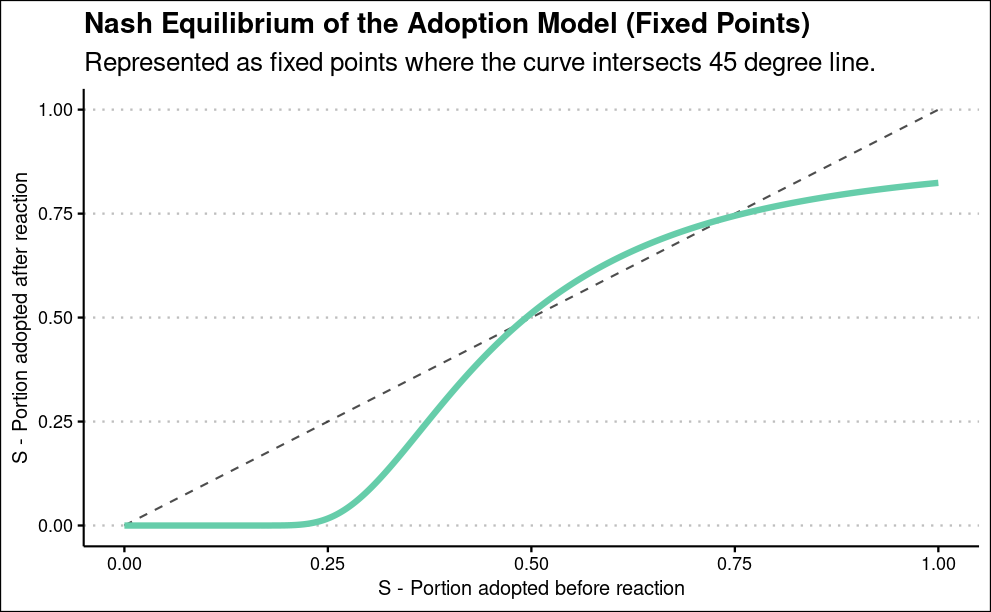
\includegraphics[width=0.7\linewidth]{adoption_curve_1.png}
    \caption{Adoption curve showing model equilibria for the following parameterization: $F_H=3$, $X=2F_H$, $\tilde{p}_H=1.2$, $\delta=0.05$, and $\gamma=0.03$. The graph shows 3 Nash equilibrium exist with this parameterization.}
    \label{fig:adopt_curve_1}
\end{figure}

In Figure \ref{fig:adopt_curve_1} the adoption curve (green) is shown over different proportions of adoption.
When the curve intersections the 45 degree line (black-dashed) that value of $S$ is a fixed point and represents a Nash equilibrium of the game.
For any input value of $S$ on the x-axis, the height of the curve (y-axis value) represents the proportion of airports that will choose adoption if all airports and airlines believe that $S$ airports will adopt. 
When the x-value differs from the y-value, it indicates that some airports and/or airlines which to change their strategy to respond better.
When the values match, however, it represents a stable point where no player desires to unilaterally deviate from their chosen strategy - a Nash equilibrium.

From the graph we see three distinct equilibrium exist.
The first and most obvious occurs as at $S = 0$ which signifies the default starting point of no airports adopting unless other airports and airlines also adopt.
The other two equilibrium are interior points at intermediate points of adoption.
It is noteworthy that in this model, 100 percent adoption is not one of the stable outcomes.

The intermediate equilibria occur at roughly 50\% and 75\% adoption.
The adoption curve remains flat from $S=0$ until after 25\% adoption after it which it finally begins to curve upward.
This may suggest that a rather large induced adoption rate is required to begin moving the to the interior equilibria with positive adoption.
Furthermore, it isn't until almost 50\% adoption that the input proportion is followed by an even higher rate of adoption.







\section{Limitations}

\section{Future Work}

\section{Conclusions}

% ------------------------------------------------------
%   BEGIN APPENDIX
% ------------------------------------------------------
\newpage
\section{Appendix}

\paragraph{Derive Demand Functions}
Starting with the tangency condition for optimality I now derive the input demand functions for cost minimization.
\begin{align}
     \; \frac{K^{\rho-1}}{\tilde{S}H^{\rho-1}} &= \frac{p_K}{p_H} \quad \text{MRTS = price ratio} \nonumber \\
     \iff\quad \frac{K^{\rho}}{\tilde{S}^{\rho/(\rho-1)}H^{\rho}} &= \left(\frac{p_K}{p_H}\right)^{\rho/(\rho-1)} \quad \text{raise both sides to }(\rho/(\rho-1) \nonumber \\
     \iff\quad K^{\rho} &= \left(\frac{p_K}{p_H}\right)^{\rho/(\rho-1)} \tilde{S}^{\rho/(\rho-1)} H^{\rho} \quad \text{raise both sides to }\rho \nonumber \\
     \iff\quad Y^{\rho}-\tilde{S}H^{\rho} &= \left(\frac{p_K}{p_H}\right)^{\rho/(\rho-1)}\tilde{S}^{\rho/(\rho-1)} H^{\rho} \quad \text{Substitute in constraint} \nonumber \\
     Y^{\rho} &= \left[ \left(\frac{p_K}{p_H}\right)^{\rho/(\rho-1)}\tilde{S}^{\rho/(\rho-1)} + \tilde{S} \right] H^{\rho} \quad \text{collect terms of } H \nonumber \\
     Y \left[ \left(\frac{p_K}{p_H}\right)^{\rho/(\rho-1)}\tilde{S}^{\rho/(\rho-1)} + \tilde{S} \right]^{-1/\rho} &= H \quad \text{raise both sides to }1/\rho \text{ to solve for }H \nonumber
\end{align}
We can now solve for the incumbent energy input demand function.
\begin{align}
    K^{\rho}\tilde{S}^{-\rho/(\rho-1)} &= \left(\frac{p_K}{p_H}\right)^{\rho/(\rho-1)} H^{\rho} \nonumber \\
    \left(\frac{p_H}{p_K}\right)^{\rho/(\rho-1)}\tilde{S}^{-\rho/(\rho-1)} K^{\rho} &= H^{\rho} \quad \text{isolate } H \nonumber \\
    \left(\frac{p_H}{p_K}\right)^{\rho/(\rho-1)}\tilde{S}^{-1/(\rho-1)} k^{\rho} &= \tilde{S} H^{\rho} \quad \text{multiply both sides by }\tilde{S} \nonumber \\
    \left(\frac{p_H}{p_K}\right)^{\rho/(\rho-1)}\tilde{S}^{-1/(\rho-1)} K^{\rho} &= Y^{\rho} - K^{\rho} \quad \text{Substitute in constraint} \nonumber \\
     \left(\frac{p_H}{p_K}\right)^{\rho/(\rho-1)}\tilde{S}^{-1/(\rho-1)} K^{\rho} + K^{\rho} &= Y^{\rho} \quad \text{Collect terms of } K \nonumber \\
     \left[ \left(\frac{p_H}{p_K}\right)^{\rho/(\rho-1)}\tilde{S}^{-1/(\rho-1)} + 1 \right] K^{\rho} &= Y^{\rho} \quad \text{Factor out } K \nonumber \\
     K^{\rho} &= Y^{\rho} \left[ \left(\frac{p_H}{p_K}\right)^{\rho/(\rho-1)}\tilde{S}^{-1/(\rho-1)} + 1 \right]^{-1} \quad \text{Isolate } K^{\rho} \nonumber \\
     K &= Y \left[ \left(\frac{p_H}{p_K}\right)^{\rho/(\rho-1)}\tilde{S}^{-1/(\rho-1)} + 1 \right]^{-1/\rho} \quad \text{raise both sides to }1/\rho \nonumber 
\end{align}
































%=========================================================
\end{document}